\let\negmedspace\undefined
\let\negthickspace\undefined
\documentclass[journal]{IEEEtran}
\usepackage[a5paper, margin=10mm, onecolumn]{geometry}
%\usepackage{lmodern} % Ensure lmodern is loaded for pdflatex
\usepackage{tfrupee} % Include tfrupee package

\setlength{\headheight}{1cm} % Set the height of the header box
\setlength{\headsep}{0mm}     % Set the distance between the header box and the top of the text

\usepackage{gvv-book}
\usepackage{gvv}
\usepackage{cite}
\usepackage{amsmath,amssymb,amsfonts,amsthm}
\usepackage{algorithmic}
\usepackage{graphicx}
\usepackage{textcomp}
\usepackage{xcolor}
\usepackage{txfonts}
\usepackage{listings}
\usepackage{enumitem}
\usepackage{mathtools}
\usepackage{gensymb}
\usepackage{comment}
\usepackage[breaklinks=true]{hyperref}
\usepackage{tkz-euclide} 
\usepackage{listings}
% \usepackage{gvv}                                        
\def\inputGnumericTable{}                                 
\usepackage[latin1]{inputenc}                                
\usepackage{color}                                            
\usepackage{array}                                            
\usepackage{longtable}                                       
\usepackage{calc}                                             
\usepackage{multirow}                                         
\usepackage{hhline}                                           
\usepackage{ifthen}                                           
\usepackage{lscape}
\begin{document}
	
	\bibliographystyle{IEEEtran}
	\vspace{3cm}
	
	\title{1.1.10.26}
	\author{EE24BTECH11059 - Yellanki Siddhanth
	}
	% \maketitle
	% \newpage
	% \bigskip
	{\let\newpage\relax\maketitle}
	
	\renewcommand{\thefigure}{\theenumi}
	\renewcommand{\thetable}{\theenumi}
	\setlength{\intextsep}{10pt} % Space between text and floats
	
	
	\numberwithin{equation}{enumi}
	\numberwithin{figure}{enumi}
	\renewcommand{\thetable}{\theenumi}
	
	
	\textbf{Question}:\\
	Find the unit vector in the direction of the sum of the vectors, $a=2\hat{i}+2\hat{j}-5\hat{k}$ and $b = 2\hat{i} + \hat{j} + 3\hat{k}$
	\\ \textbf{Solution: }\\
	\begin{table}[h!]    
		\centering
		

		\caption{}
	\end{table}\\
	To calculate the $c$,
	\begin{align}
		a+b = \myvec{2 \\ 2 \\ -5} + \myvec{2 \\ 1\\3}  = \myvec{4 \\ 3\\-2}\label{eq1.1.10.26.1}
	\end{align}
	Calculating $\norm{a+b}$, using the formula $\norm{c}=\sqrt{c_x^2 + c_y^2 + c_z^2}$
	\begin{align}
		\norm{a+b} = \sqrt{4^2 + 3^2 + 2^2}=\sqrt{29} \label{eq1.1.10.26.2}
	\end{align}
	$\therefore$ $c$ is,
	\begin{align}
		c = \frac{a+b}{\norm{a+b}} = \frac{1}{\sqrt{29}}\myvec{4 \\ 3\\-2} \label{eq1.1.10.26.3}
	\end{align}
	\begin{figure}[h]
		\centering
		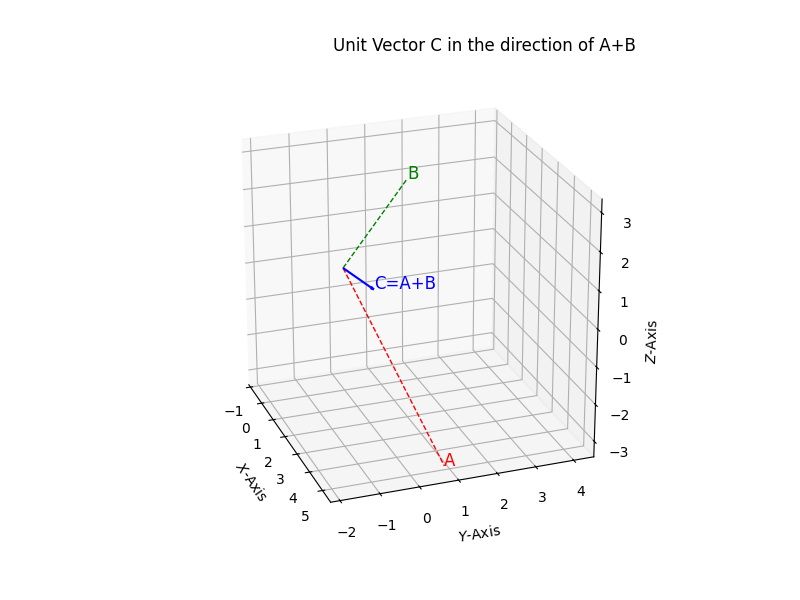
\includegraphics[width=0.7\linewidth]{figs/fig1.png}
		\caption{}
		\label{graph}
	\end{figure}
	
	
	
\end{document}  







